% UNIT: Psychology of Concepts and Categories
\chapter{Psychology of concepts and categories}
\label{chap:concepts_categories}

In this Chapter we discuss about categories in sensation/perception (non-semantic categories, Section \ref{sec:categories}) and conceptual structure (words and concepts, Section \ref{sec:conceptual_structure}).

\section{Categories and categorical perception}
\label{sec:categories}

Categorical perception is the phenomenon in which people perceive stimuli from different categories as more different from each other than stimuli from within the same category. This is useful as it introduces invariance in response with respect to a functionally defined category, allowing for rapid prediction, efficient memory, and compression.

\boxc{How we know categorical representation exists}{
A demonstrating experiment consists in:
\begin{itemize}
    \item selecting a set of stimuli that uniformly covers a certain physical domain (e.g. sound freq 100Hz-8000Hz),
    \item select an objective distance measure so that the space is partitioned in intervals; e.g. distance in frequency space (applicable to both sounds and colors),
    \item select a method for operationalizing human similarity (e.g. similarity judgments, generalization, confusion [same/different]),
    \item in one procedure, assign all stimuli to categories (e.g. assign all stimuli to color names); in a second, obtain similarity judgments for within-category vs. between-category pairs, or ask for categorization, and evaluate if the boundary is fuzzy or not (e.g. how much objects are considered similar when belonging to the same category, and when to different categories)
\end{itemize}
}

\subsection{Categorical perception in audition}
In auditory stimuli, there is discrimination between speech sounds. People have a sharper discrimination boundary between sounds that are perceived as belonging to different phonetic categories than between sounds that are perceived as belonging to the same category.
For experimenting, we use as objective dimension the \textbf{Voice Onset Time} (VOT) of consonants (i.e. the timespan between the start of the consonant and the start of sound emitted by vocal cords). The discrimination performance is simply a ``same/different" judgment. We present consonants such as /b/ and /p/. A fixed-size physical difference in VOT, that is easily discriminated when it straddles the boundary between two categories (labeled as /b/ or /p/), produces \textit{chance} discrimination performance when both tokens come from the same category (either both /b/ or both /p/); results are in Figure \ref{fig:bapa}.

\textbf{Within phonetic category}, two \textbf{different stimuli sound the same} (see \notedv Eimas et al. (1971)).\\

Prior categories aid online processing via categorical perception, in a sort of \textit{experience-dependent learning}; related phenomena are:
\begin{itemize}
    \item \textit{Change deafness}, Vitevitch (2003): participants repeat words presented by a speaker. Halfway through study, the speaker changed. Only 40\% of participants noticed the change.
    \item \textit{Sine-wave speech}: phonetic categories/expectations can be considered \textit{priors} on sounds, impacting whether a stimulus is perceived as speech (e.g. if you previously listen to a voice and then hear a sound which is not speech, but has some correlation to the previous voice, you can ``hear" the words).
    \item \textit{McGurk Effect}: the categorization of sounds is not only an auditory task, since our brain combines multimodal inputs (e.g. also from vision).
\end{itemize}

\begin{figure}
    \centering
    \captionsetup{width=.8\linewidth}
    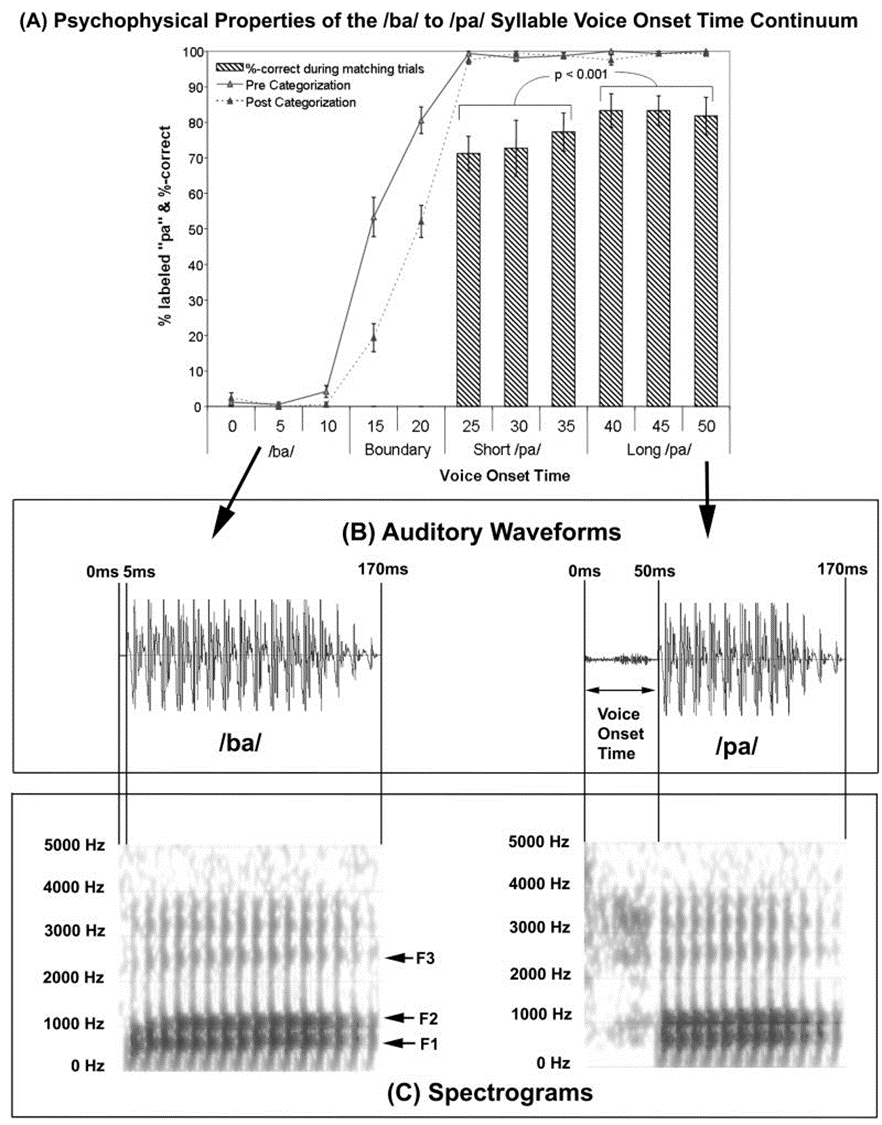
\includegraphics[width=0.8\linewidth]{images/vot.png}
    \caption{For the experiment, they created a range of stimuli with VOT between 5ms and 50ms (which are the standard values for respectively /ba/ and /pa/).
    In \textbf{(A)} are the results, with the percentage of responders hearing a /pa/ sound. We see the shift is between 10ms and 25ms}
    \label{fig:bapa}
\end{figure}

\boxl{Eimas et al. (1971)}{
They observed 4-month old sucking rate on pacifier (notice that a higher rate is interpreted as more surprise/interest). They examined the rate as function of relation between current and previously heard stimuli, in particular they presented two stimuli with VOT differing by 20ms. In one condition (labeled ``D") the difference straddled (on two sides of) the border of a phonetic boundary (stimuli perceived as ``b" and ``p" by adults). In another condition ``S" they belonged to the same phonetic category.\\

See Figure \ref{fig:eimas} for more details.
}

\begin{wrapfigure}[20]{r}{0pt}
  \begin{subfigure}{.22\textwidth}
  \centering
    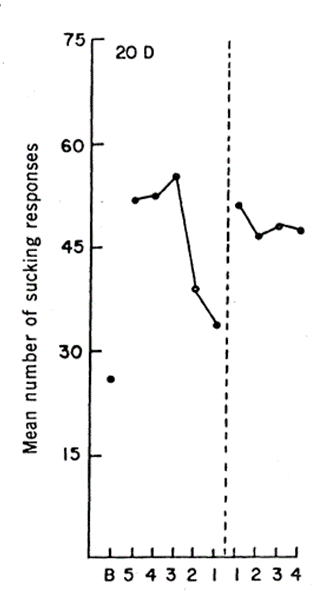
\includegraphics[height=5.5cm]{images/eimas_a.png}
    \caption{}
  \end{subfigure}%
  \begin{subfigure}{.2\textwidth}
  \centering
    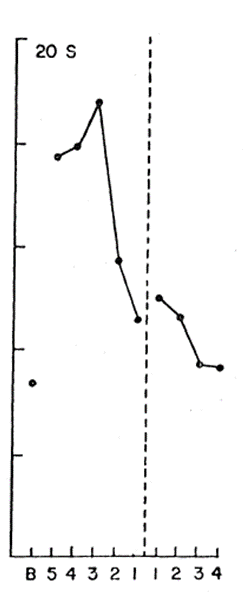
\includegraphics[height=5.5cm]{images/eimas_b.png}
    \caption{}
  \end{subfigure}
  \caption{5 min of habituation precede a 20 ms VOT change, either within the same \textbf{(a)} or across \textbf{(b)} phonetic category; habituation consists in hearing the /ba/ sound. This proves how 4-month-old children already have the auditory \textbf{categorization} enabling them to distinguish between /b/ and /p/ sounds.}
    \label{fig:eimas}
\end{wrapfigure}

Brain areas coding for \textbf{low-level} representations are \textbf{not influenced} by such categorization, while those coding for high-level representations do.

\subsection{Categorical perception in vision}
In categorical perception for color, discrimination of items that cross category boundaries is better (faster, more accurate) than when the items are within the same color category. Notice that color category is \textbf{linguistic} \notet.
For example, it is easier to distinguish between a green stimulus and a blue stimulus than between two stimuli within the same category (two shades of green), who are \textbf{spaced at the same distance}.
\osst{Practical note: color differences in terms of discriminability can be equated across between-category and within-category comparisons by using the \textit{Commision Internationale de L’Eclairage} (CIE) values.}

\textbf{Color categories are not universal}, and thus \textbf{categorical perception depends on language} (see \notetv Robertson et al. (2000)).

\boxl{Robertson et al. (2000)}{
A stone-age tribe Berinmo uses ``\textit{nol}” as the color name that in English fall under both green and blue, so they have no categorical perception at the boundary between green and blue (no boundary in their language). On the contrary, they have a category boundary between ``\textit{nol}" and ``\textit{wor}'' that does not exist in English as both sides are green. Berinmo people exhibit better discrimination of 32 cross-category items than 32 within-category items at the boundary between \textit{nol} and \textit{wor}. English speakers do not show categorical perception at this boundary.
}

\section{Conceptual structure}
\label{sec:conceptual_structure}

\subsection{Theory on words and concepts}
The typical approach is to assume that words are associated with concepts or a network of conceptual representations.
We need to first have a good theory of what the conceptual structure is like, and then we can see how this structure is used to represent meaning when referred to by words.
Ultimately, a word is a sound or written pattern, and it is generally assumed that a single word corresponds to a single concept (this assumption would help with word-embedding models), but there are complications.

There is evidence proving that \textit{form-to-meaning mapping} is not 1-to-1. This evidence is called \textbf{polysemy}: a phenomenon where a single word can have multiple meanings depending on the context in which it is used, such as ``cinema" which can refer to different things in different contexts (e.g. \textit{American cinema is naïve} vs \textit{This cinema is ugly}).

According to Murphy, it is impossible for a single concept to fully capture the meaning of a polysemous word; the process of meaning extension is not a result of \textit{natural change} (chaining) but a matter of \textbf{online derivation}. Online derivation does not prevent information from being also stored somewhere, at least for a short time, in order to understand the nearby context more effectively. Indeed, Klein and Murphy (2001) found evidence suggesting that the different senses of polysemous words can be stored, as they observed priming effects when a word was used twice in the same sense, and interference effects when the sense was switched.

Another possibility is that a word specifies a set of potentials that is then refined by context to determine which sense is intended.\\

We found out that \textbf{words are not concepts}. Such distinction between \textit{meaning} and \textit{lexical form} is also proven by \textit{anomia}. It is a type of \textit{aphasia} that results in the inability to retrieve the lexical form of a concept for production, even though the ability to recognize or define the term is maintained.


\subsection{Representing the meaning of concepts in the brain}

